

%%%%%%%%%%%%%%%%%%%%%%%%%%%%%%%%%%%%%%%%%%%%%
\graphicspath{{/media/data/Work/cnstellate/golgi/}{/media/data/Work/Responses/}{/media/data/Work/cnstellate/Responses/}{../figures/}{./gfx/}}
%%%%%%%%%%%%%%%%%%%%%%%%%%%%%%%%%%%%%%%%%%%%%

\section[Golgi Cell Model]{Golgi Cell Model: Optimisation using
  monotonic rate-level responses in marginal shell units}
\label{sec:golgi-cell-model}
% Modelling in the auditory periphery has benefited extensively from
% the work of Liberman, Greewood, Patterson, Young, Sachs and others,
% in acoustic \it{in vivo} experiments.

\subsection{Golgi Cell Literature}

The source of GABAergic inputs to cells in the mammalian CN is
somewhat contentious. Despite studies showing that GABAergic inputs to
the CN generally arise in the peri-olivary regions of the medulla in
cats \citep{OstapoffBensonEtAl:1997} and birds
\citep{LachicaRubsamenEtAl:1995,YangMonsivaisEtAl:1999}, slice
preparations of the isolated murine VCN have shown sensitivity to
bicuculine in TS and DS cells \citep{FerragamoGoldingEtAl:1998a}.  The
only known source of GABA intrinsic to the VCN are the golgi cells of
the granule cell domain (GCD) overlying the VCN
\citep[Fig.~\ref{fig:CNdiagram}]{Mugnaini:1985,FerragamoGoldingEtAl:1998}.
The presence of GABAergic inputs to TS, DS and TV cells has been
verified by labeled terminals adjacent to the soma and dendrites
\citep{SmithRhode:1989,AwatramaniTurecekEtAl:2005,BabalianRyugoEtAl:2003}
and release from inhibition in their response areas with
ionotopopheretic application of the GABA antagonist, bicuculine
\citep{EvansZhao:1998,CasparyBackoffEtAl:1994,BackoffShadduckEtAl:1999,FerragamoGoldingEtAl:1998a}.

Other studies in the rat cochlear nucleus relating to the Golgi cell or GABA:
\begin{itemize}
\item \citep{MugnainiOsenEtAl:1980} Fine structure of granule cells
  and related interneurons (termed {Golgi} cells) in the cochlear
  nuclear complex of cat, rat and mouse
\item GABAa expression in the rat brainstem  \citep{CamposCaboEtAl:2001}
\item \citep{Alibardi:2003a} Ultrastructural distribution of
  glycinergic and {{GABAergic}} neurons and axon terminals in the rat
  dorsal cochlear nucleus, with emphasis on granule cell areas
\item \citep{AwatramaniTurecekEtAl:2005} Staggered {Development} of
  {GABAergic} and {Glycinergic} {Transmission} in the {MNTB}
\end{itemize}

Role of GABA in the VCN
\begin{itemize}
\item Effects of microiontophoretically applied glycine and {GABA} on
  neuronal response patterns in the cochlear nuclei
  \citep{CasparyHaveyEtAl:1979}
\end{itemize}

\citep{Alibardi:2003a} rat CN complex -> Golgi-stellate cells
(fusiform layer: 2) in DCN contact granule and unipolar brush cells


Inputs to golgi cells are more complicated than VCN cells in the core
regions. Golgi cells are sparse in the GCD, surrounded by the many,
smaller excitatory granule cells, that form small en passant
endings. Type II ANFs create diffuse glutamatergic release sites in
the GCD \citep{HurdHutsonEtAl:1999,BensonBrown:2004} that may
stimulate NMDA glutamate receptors in golgi cells
\citep{FerragamoGoldingEtAl:1998a}.


Extracellular recordings from the GCD by \citet{GhoshalKim:1997}, are most likely from golgi
cells since granule cell somata are less than  $10 \mu m$ and very
narrow axons. The majority of recorded
units showed a monotonic increase in firing rate with increasing sound
intensity \citep{GhoshalKim:1997}. 


\medskip{}

The lack of extensive experimental data meant that a phenomenological model
would be preferred over the Hogkin-Huxley type neural model. A number of steps
were taken to investigate the golgi cell model.

The known GABAergic input to VCN units comes primarily from the superior olive
(ref), but the presence of active GABA synapses in isolated VCN slices by
\citet{FerragamoGoldingEtAl:1998} led to further investigation of
golgi cells in the granule cell domain. \citet{FerragamoGoldingEtAl:1998a}
showed that golgi cells have a classic type-I current
response, which suggest they integrate inputs, and their response to
AN shocks were delayed by approximately 0.7~ms relative to the core
VCN units .  Ghosal and Kim
\citet{GhoshalKim:1997} examined the VCN marginal shell in cats (equivalent to the
GCD in mice) that golgi cells provide some sort of
automatic gain control to the principle VCN units, through their monotonic
responses to tones and noise.

\medskip{}

% (Reference) showed that in adult animals high-spontaneous rate ANFs do not
% project to the GCD; they do show that low-spontaneous rate ANFs do project into
% the GCD, albeit more profusely than in the core on the VCN.
   

\begin{figure}[htb]
  \centering
\resizebox{0.8\textwidth}{!}{\includegraphics{NoFigure}}
%  \resizebox{0.8\textwidth}{!}{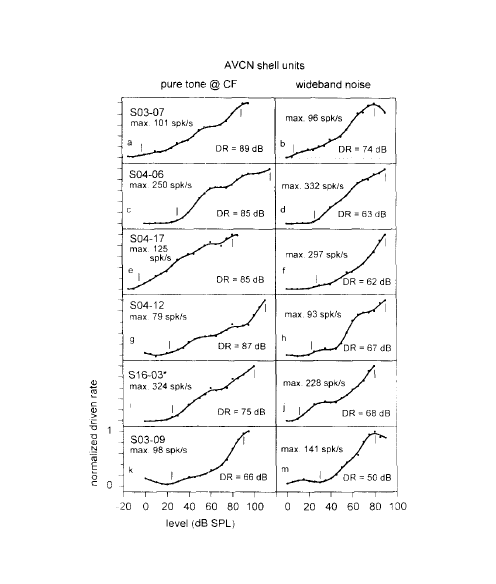
\includegraphics{GhoshalKim}}
\caption{Rate level response of unit S03-07 (CF 21~kHz) from Fig2
  \citep{GhoshalKim:1997} }
\end{figure}


\newpage
\subsection{Implementation}
\vspace{1ex}
% - A ------------------------------------------------------------------------


In the creation of the golgi cell model, we can reduce the explicit
responses of Golgi cells down to:\begin{itemize}\setlength{\itemsep}{-1em}
\item type-I~current clamp response,
\item monotonic response to tones and noise, and
\item delay from ANFs of approx. 0.7~ms relative to the core VCN units.
\end{itemize}

In Chapter~\ref{sec:GAChapter} and previous publications \citep{EagerGraydenEtAl:2006a}


Monotonic rate-level data from GCD in VCN \citep{GhoshalKim:1996} unit S03-07
(CF 21~kHz) was used to optimise parameters ${\rm golgi\_spon}$, \wLSRGLG,
\wHSRGLG, and  \sANFGLG\@.  The optimisation method was a default  using the principle-axis method.


To summarise the neural model used in this optimisation, I have
reduced the information to tabular format as suggested by
\citet{NordlieGewaltigEtAl:2009}.



due to its replication of granule cells in the model. weight for LSR \wLSRGLG and HSR \wHSRGLG are determined  for all synapses, number \nLSRDS and \nHSRDS, delay \dANFGLG added to smoothing function to ensure conductance and dendritic filtering are included.

** Golgi Cell Model :  Key design factors
 - Choosing neural model: HH-type or Poisson
 - Problem of monotonic excitation at low level
  - added HSR to model to avoid added computation of MSR
 - Spread of ANF to GCD ARE broader than core VCN
  - are we spoiling the broth too early? 


\begin{figure}[hp!]
  \centering
  \includegraphics[width=0.9\textwidth,trim=0 110mm 1 55mm]{gfx/GolgiDiagram}
  \caption{ The golgi instantaneous-rate profile was generated using ANF
    profiles. $\mu$ and $\sigma$ control the spread of connections
    across frequency channels, and $\mathbf{w}$ is
    the weighted sum of HSR and LSR instantaneous-rate vectors,
    $\alpha$ is the synaptic and dendritic smoothing function.}
\end{figure}


\noindent\begin{tabularx}{\linewidth}{|l|X|}\hline %
\hdr{2}{A}{Model Summary}\\\hline 
 \textbf{Populations}   & ANF(HSR,LSR) and Golgi \\\hline 
   \textbf{Topology}    & Tonotopic - 100 frequency channels based on Rat basilar membrane \citep{Greenwood:1990} and audiogram \citep{HeffnerKoayEtAl:2001}\\\hline
 \textbf{Connectivity}  & Place-based Gaussian spread of connections \\\hline
 \textbf{Neuron model}  & ANFs: phenomenological instantaneous-rate Poisson model \citep{ZilanyBruceEtAl:2009} \\
& Golgi: instantaneous-rate Poisson model developed from ANF inputs\\\hline
\textbf{Channel models} & --- \\\hline 
\textbf{Synapse model}  & alpha function smoothing kernel \\\hline
\textbf{Input}      & Pure tones (21 kHz, 50 ms, 5 ms on/off ramp, 20 ms delay), 0-100 dB SPL  \\\hline
 \textbf{Measurements}  & Mean rate, spike activity \\\hline
\end{tabularx}

% - B ------------------------------------------------------------------------
\noindent\begin{tabularx}{\linewidth}{|l|X|X|}\hline %{\linewidth}
\hdr{3}{B}{Populations}\\\hline
  \textbf{Name}   & \textbf{Elements} & \textbf{Number} \\\hline
    HSR     & \citeauthor{ZilanyBruceEtAl:2009}  model        & $N_{\text{HSR}} = 50$ per freq.\ channel \\\hline
    LSR     & \citeauthor{ZilanyBruceEtAl:2009} model        & $N_{\text{LSR}}= 20$  per freq.\ channel \\\hline
    GLG     & Instantaneous rate Poisson model, spike-generator with refractory effects & $N_{\text{GLG}}= 1$  per freq.\ channel  \\\hline
\end{tabularx}
\vspace{1ex}

% - C ------------------------------------------------------------------------------
\noindent\begin{tabularx}{\linewidth}{|l|l|l|X|}\hline
\hdr{4}{C}{Connectivity}\\\hline
\textbf{Name} & \textbf{Source} & \textbf{Target} & \textbf{Pattern} \\\hline
  \multirow{2}{*}{$\textrm{ANF} \to \textrm{GLG}$} & LSR & Golgi &
  Gaussian spatial spread, centered at CF, variance determined by \sLSRGLG \\
 & HSR & Golgi & Fixed Gaussian spatial spread, centered at CF (\sHSRGLG =) \\\hline
 \end{tabularx}

\vspace{1ex}
% - D ------------------------------------------------------------------------------
\noindent\begin{tabularx}{\linewidth}{|l|X|}\hline
\hdr{2}{D}{Neuron and Synapse Model}\\\hline
            \textbf{Name}             & Golgi Phenomenological Model \\\hline
            \textbf{Type}             & Poisson instantaneous-rate model, ANF instantaneous rate input\\\hline
\multirow{4}{*}{\textbf{Golgi Model}} & $\mathbf{w}_{LSR} = N(\textrm{CF channel},\sLSRGLG)$,  $\mathbf{w}_{HSR} = N(\textrm{CF channel},\sHSRGLG)$  \\ 
                                      & $w(i,j) = \frac{1}{\sigma \sqrt{2\pi}} \exp \left\{-\frac{(i-j)^2}{2\sigma^2}\right\}, i,j \in [0,nchannels-1]$ \\
                                      & $\mathbf{g}_i = \sum^{i} w_{LSR}(i)\mathbf{L}_i + w_{HSR}(i)\mathbf{H}_i$ \\
                                      & $\mathbf{G}_i = \mathbf{g}_i * \alpha$  \\ \hline
\end{tabularx}
%\end{eqnarray}
% $\mathbf{w}_{LSR} = N(\textrm{CF channel},\sLSRGLG)$,  $\mathbf{w}_{HSR} = N(\textrm{CF channel},\sHSRGLG)$  \\ 
% &\texttt{for \textit{i}=0, nchannels} \\
% &	$\quad\mathbf{x}_i = \mathbf{w}_{LSR}(i)\cdot\mathbf{LSR}_i+\mathbf{w}_{HSR}(i)\cdot\mathbf{HSR}_i$ \\
% &\texttt{end} \\
% &	$\mathbf{x} = \mathbf{x}_i\circledast\mathbf{a}$  \texttt{//Convolve profile with Alpha kernel}\\\hline
% \multirow{3}{*}{\textbf{Spiking}} &
%    If $V(t-)<\theta \wedge V(t+)\geq \theta$
% \vspace*{-1ex}
% \begin{enumerate}\setlength{\itemsep}{-0.5ex}
% \item set $t^* = t$
% \item emit spike with time-stamp $t^*$
% \end{enumerate}
% \vspace*{-4ex}\rule{1em}{0em}
% \\\hline


% - E -----------------------------------------------------------------------------
\vspace{1ex}
\noindent\begin{tabularx}{\linewidth}{|l|X|}\hline %
\hdr{2}{E}{Input/Output}\\\hline 
\textbf{Input Stimulus} & Rate Level function, 21~kHz tone at SPL -15
to 85 dB (20 ms delay, 2ms cosine squared on/off ramp)\\\hline 
\textbf{Measurements}        & Mean rate of instantaneous rate profile or PSTH sampled from Poisson spike-generator (25 repetitions). \\\hline
\end{tabularx}
\vspace{1ex}



\noindent\begin{tabularx}{\linewidth}{|X|c|c|c|}\hline %{\textwidth}
\hdr{4}{F}{Optimisation} \\ \hline 
     \textbf{Parameters}      &  \textbf{Name}   & \textbf{Range} & \textbf{Best Values} \\\hline 
   Spatial spread $\ANFGLG$     &     $\sANFGLG$     &     [0,10]     & 2.48 \\\hline 
Dendritic Filter time constant& $\tau_{\ANFGLG}$ &    [0,20] ms   & 5.01\\\hline 
     Weighted sum of HSR      &    $\wHSRGLG$    &      [0,5]     & 0.517 \\\hline 
     Weighted sum of HSR      &    $\wLSRGLG$    &      [0,5]     & 0.0487\\\hline 
      Spontaneous Rate        &  \texttt{golgi\_spon} &  [0,50] sp/ms  & 3.73 \\\hline
\end{tabularx}




% \includegraphics[width=0.6\textwidth,angle=-90]{GolgiRateLevelActualFit}\\
% \caption{Optimisation Results for Golgi Model using Rate Level data
%   from }\label{Ch3:fig:GolgiFit}
% \includegraphics[width=0.8\textwidth]{GolgiRateLevel}\\
% \caption{Optimisation Results for Golgi Model using Rate Level data
%   from }\label{Ch3:fig:GolgiRL}

% \includegraphics[width=0.8\textwidth]{golgi_RateLevel_opt}\\
% \caption{Optimisation Results for Golgi Model using Rate Level data
%   from }\label{Ch3:fig:GolgiRL}
% \includegraphics[width=0.8\textwidth,angle\todo=-90]{GolgiRateLevel2}\\
% \caption{Optimisation Results for Golgi Model using Rate Level data
%   from }\label{Ch3:fig:GolgiRL}

\clearpage
\subsection{Results}
Fig. 4: Golgi model (Green) and spike based output (Pink) was used to
fit the experimental data of unit S03-07 (CF 21~kHz) from
\citep{GhoshalKim:1996} (Red).  LSR mean rate (Blue) of 21~kHz unit is
monotonic with a high threshold.



\begin{figure}[htb]
  \centering \turnbox{90}{\small{Rate (sp/s)}}
%  \resizebox{0.8\textwidth}{!}{\includegraphics[angle=-90]{GolgiRateLevel2}}\\
  \caption{Rate Level (dB SPL)}
\end{figure}


\textbf{Error} 0.021 (MSE re max rate)



% \clearpage \newpage
\section{Verification}
\subsection{Tone Response}

\begin{figure}[h]
  \centering\resizebox{0.95\textwidth}{!}{%
    \includegraphics{RateLevel/psthsingle90.3.eps}%
    \includegraphics{RateLevel/G_ratelevel.eps}}
\end{figure}
\begin{figure}[h]
  \centering\resizebox{0.95\textwidth}{!}{%
    \includegraphics{RateLevel/response_area.3.eps}%
    \includegraphics{RateLevel/response_area_log2.3.eps}}
\end{figure}
\begin{figure}[h]
  \centering\resizebox{0.95\textwidth}{!}{%
    % \includegraphics{RateLevel/response_area.3.eps}
    \includegraphics{RateLevel/psthall90.3.eps}%
    \includegraphics{RateLevel/psthVlevel.3.eps}}
\end{figure}



\clearpage
\subsection{Noise Response}
\begin{figure}[h]
  \centering\resizebox{0.95\textwidth}{!}{%
    \includegraphics{NoiseRateLevel/psthsingle120.3.eps}%
    \includegraphics{NoiseRateLevel/G_ratelevel.eps}}
\end{figure}
\begin{figure}[h]
  \centering\resizebox{0.95\textwidth}{!}{%
    \includegraphics{NoiseRateLevel/response_area.3.eps}%
    \includegraphics{NoiseRateLevel/response_area_log2.3.eps}}
\end{figure}
\begin{figure}[h]
  \centering\resizebox{0.95\textwidth}{!}{%
    % \includegraphics{RateLevel/response_area.3.eps}
    \includegraphics{NoiseRateLevel/psthall90.3.eps}%
    \includegraphics{NoiseRateLevel/psthVlevel.3.eps}}
\end{figure}


\clearpage
\subsection{Masked Noise and Tone}
\begin{figure}[h!]
  \centering\resizebox{0.95\textwidth}{!}{\includegraphics{MaskedRateLevel/psthsingle90.3.eps}\includegraphics{MaskedRateLevel/G_ratelevel.eps}}
\end{figure}
\begin{figure}[h!]
  \centering\resizebox{0.95\textwidth}{!}{%
    \includegraphics{MaskedRateLevel/response_area.3.eps}%
    \includegraphics{MaskedRateLevel/response_area_log2.3.eps}}
\end{figure}

\begin{figure}[h!]
  \centering\resizebox{0.95\textwidth}{!}{%
    % \includegraphics{RateLevel/response_area.3.eps}
    \includegraphics{MaskedRateLevel/psthall90.3.eps}%
    \includegraphics{MaskedRateLevel/psthVlevel.3.eps}}
\end{figure}
\clearpage
\subsection{Masked Response Area}
\begin{figure}[h!]
  \centering\resizebox{0.95\textwidth}{!}{%
    \includegraphics{MaskedResponseCurve/psthsingle5810.3.eps}%
    \includegraphics{MaskedResponseCurve/G_masked.eps}}
\end{figure}
\begin{figure}[h!]
  \centering\resizebox{0.95\textwidth}{!}{%
    \includegraphics{MaskedResponseCurve/response_area.3.eps}%
    \includegraphics{MaskedResponseCurve/response_area_log2log2.3.eps}}
\end{figure}

\begin{figure}[h!]
  \centering\resizebox{0.95\textwidth}{!}{%
    % \includegraphics{RateLevel/response_area.3.eps}
    \includegraphics{MaskedResponseCurve/psthall5810.3.eps}%
    \includegraphics{MaskedResponseCurve/psthVmod.3.eps}}
\end{figure}
\clearpage


% \todo{add stuff here}



% % %%%%%%%%%%%%%%%%%%%%%%%%%%%%%%%%%%%%%%%%%%%%%%%%%%%%%%
% \bibliographystyle{plainnat}%bmc_article} % Style BST file
% \bibliography{../manuscript/bib/MyBib}
 
% \end{document}













%%% Local Variables: 
%%% mode: latex
%%% TeX-master: "SimpleResponses"
%%% TeX-PDF-mode: nil
%%% End: 
